% ##################################################################################################################
\chapter{Caracas}
\label{ch:caracas}
\hfill \textbf{Authors:} Walter J. Hernández B., Héctor E. Navarro U.

\editdone{This text has undergone the professional edit. Please no grammatical changes anymore! They are most-probably wrong.}
% ##################################################################################################################

Capital of the country, Caracas is the largest city in Venezuela, with serious vehicle traffic issues. Its daily estimated circulation of 1.5\,million units represents three times the load originally estimated for the city's growth. %One of the current main issues for planning is 
Despite the lack of official statistics, it is possible to estimate the amount of Caracas' traffic using other national figures, such as the \emph{Time Travel Index} employed by the \citet{fhwa2013}. This index estimates approximately 50\,\% longer than \emph{free-flow travel} to traverse inner city circles and 75\,\% around  metropolitan areas. This is in stark contrast to an average city in the US, which normally does not go beyond 35\,\%, even in the worst case.

Apart from obvious budget-related deficits these delays cause in work force productivity for companies and organizations, the country itself loses an estimated \$2.1\,billion per year. This includes the precious subsidies that have helped to maintain the country's world lowest prices of gas for decades (\citet{wilson2008}); \$1\,billion could be saved by reducing the average circulation time by just 30\,minutes. Equally important, the accompanying significant reduction in \gls{co2} emissions would help meet greenhouse targets for the country.

In recent years, several measures have been initiated to cope with increased traffic in Caracas:

\begin{itemize}\styleItemize
\item \gls{hov} lanes (\citet{turnbull1990}), implemented in a \emph{contraflow} fashion to increase traffic flow on central roads and highways.

\item Bus lanes for rapid bus trips and bicycle lanes, to stimulate use of alternative means of transport.

\item Shifting job starting hours to non-peak times and increasing the number of at-home working hours for certain types of jobs, to cut back vehicle use and general costs to public transport.
\end{itemize}

In addition to the these measures, other mechanisms could be implemented, such as weekday circulation restrictions (\eg based on license plate numbers) and smart traffic lights. Especially in the case of smart traffic devices and planning of special lanes, careful study and simulation of traffic patterns must be undertaken. To help achieve this, a software tool was envisioned with the following objectives:

\begin{itemize}
 \item To envision creation and editing of traffic networks on \gls{matsim} format and assign validation points to the network.

\item To study and analyze simulation results, especially the traffic volumes assigned to roads.

\item To translate data obtained in \gls{od} format for input to \gls{matsim}.

\item To run the simulations and validate outputs in order to calibrate the parameters involved.
\end{itemize}

The tool was tested with real data traffic in a Caracas area ``Los Cortijos'' (Figure~\ref{fig:caracas1left}), one of the most heavily traveled zones on the city's east side. The simulation model belongs to the \emph{microscopic} category, made by \citet{gartner2001}, since only individual elements are taken into account (\ie vehicles).

 %------------
\createfigure%
{An area of ``Los Cortijos'' in Caracas, Venezuela}%
{An area of ``Los Cortijos'' in Caracas, Venezuela}%
{\label{fig:caracas1}}%
{%
 \createsubfigure%
 {Snapshot obtained from \gls{osm}}
 {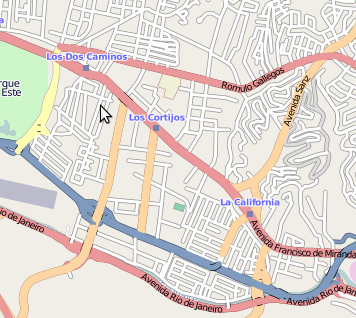
\includegraphics[width=0.35\textwidth, angle=0]{./scenarios/figures/caracas0.png}}
 {\label{fig:caracas1left}}
\createsubfigure%
 {Three snapshots of a simulation ran in \gls{matsim} between 6:00 and 6:30\,am, depicting the increasing traffic in the zone}
 {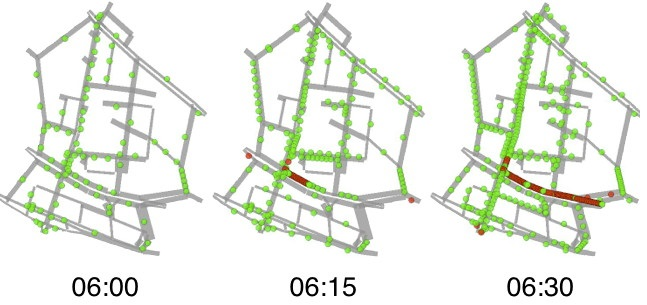
\includegraphics[width=0.64\textwidth, angle=0]{./scenarios/figures/caracas1.jpg}}
 {\label{fig:caracas1right}}
}%
{}
 %------------

The network was created by using data from \gls{osm}, then manually modifying it (\ie setting correct speed, capacity attributes) based on information delivered by a company conducting a study in the same area. Demand was given in a \gls{od} matrix by the same company, but only for the morning period. As the area researched is mainly a consuming zone in the morning and a producing zone in the afternoon, values from the \gls{od} matrix were used to create day-plans for the agents. An initial departure time around 7:30\,am was assigned to the plans.

Several scenarios with different re-planning rates were run to test how much agents have to change their departure time in the morning to allow the network to accommodate all travel demand. Figure~\ref{fig:caracas1right} shows how traffic jams builds up in the scenario where simulated demand best matches real-world traffic count.

Figure~\ref{fig:caracasA} shows the interface of the tool providing options to: load a map from \gls{osm}, load a network from \gls{matsim}, load counters (blue dots in the map image), save the map and export to a shape file (an open file format for \gls{gis} systems).

 %------------
\createfigure%
{Interface of the software tool developed in \gls{java} showing the area studied}%
{Interface of the software tool developed in \gls{java} showing the area studied. Blue dots over the roads in the map represent the counters positioned in the area to capture vehicle flow used as input for the simulation}%
{\label{fig:caracasA}}%
{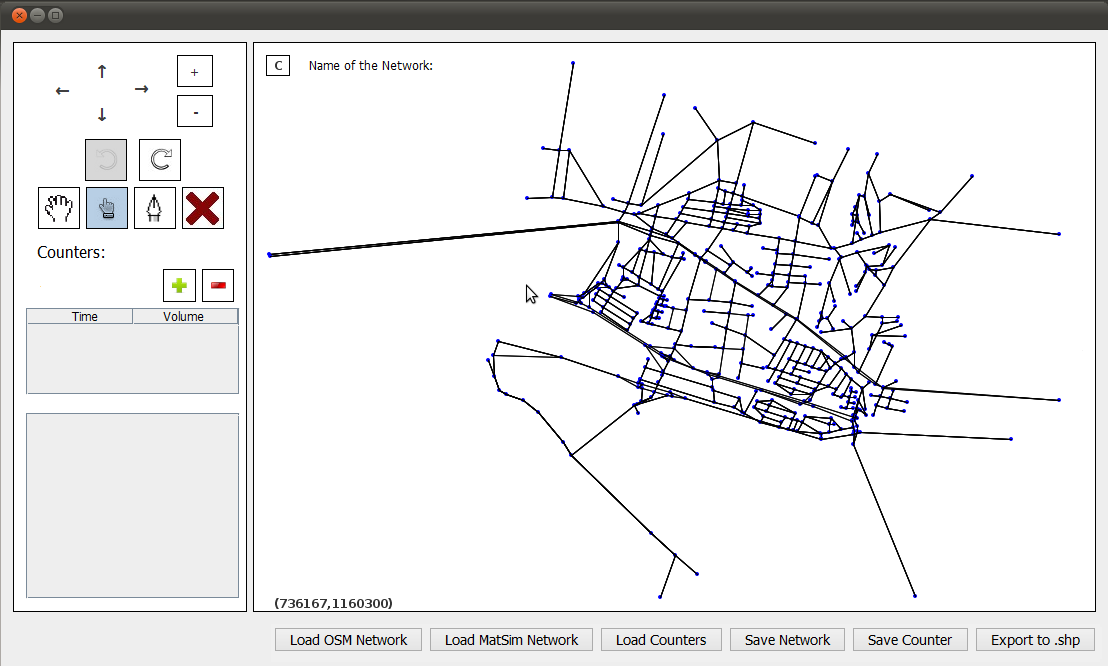
\includegraphics[width=0.99\textwidth, angle=0]{./scenarios/figures/caracasA.png}}%
{}
 %------------

Figure~\ref{fig:caracasBleft} shows an image output of the same area after running a simulation generated with \gls{matsim} and including a vehicle-density color map. Figure~\ref{fig:caracasBright} shows a sample score graph from one of the many tests run: \emph{avg. trip time} of 02h:06m:38s and \emph{avg. distance per agent} of 1727.83\,meters; \textit{total run time} of the simulation was 41\,minutes 56\,seconds.

 %------------
\createfigure%
{Simulation results}%
{Simulation results}%
{\label{fig:caracasB}}%
{%
 \createsubfigure%
 {A snapshot of the area at 7:00\,am  with a color map for vehicle flow}
 {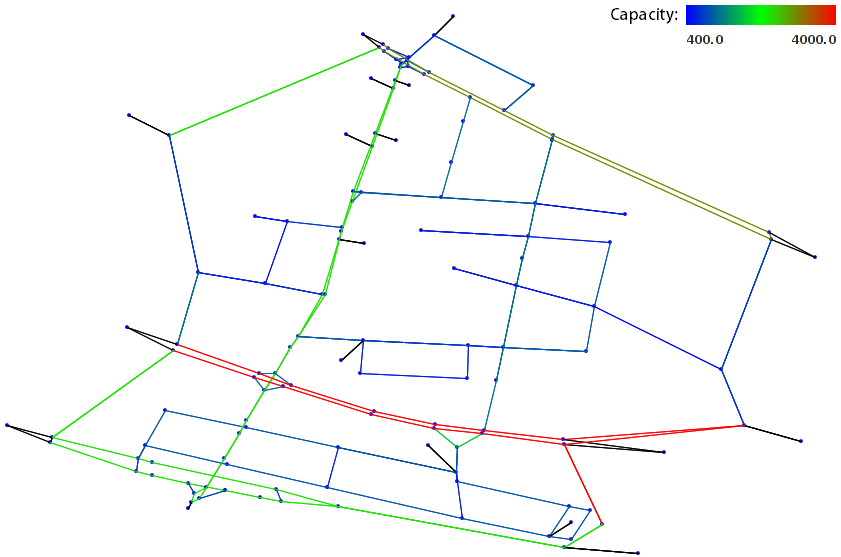
\includegraphics[width=0.49\textwidth, angle=0]{./scenarios/figures/caracasB1.png}}
 {\label{fig:caracasBleft}}
\createsubfigure%
 {\gls{matsim} sample score statistic for one of the scenarios defined}
 {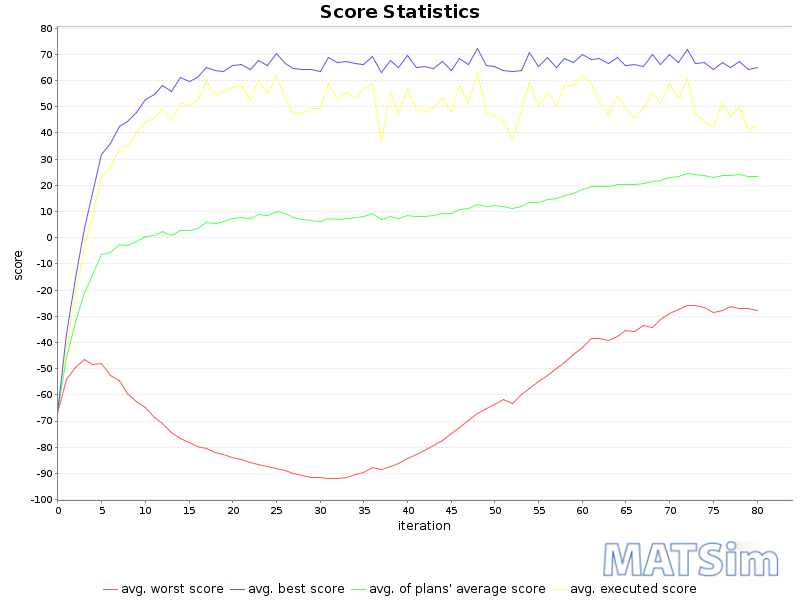
\includegraphics[width=0.49\textwidth, angle=0]{./scenarios/figures/caracasB2.png}}
 {\label{fig:caracasBright}}
}%
{}
 %------------

In spite of differing approaches between the company's study and our own results, through simulations, the numbers were quite similar with a range of difference not exceeding 3\,\% (-0.42\,\% to 2.52\,\%). Examining these promising results, but also the limitations encountered, the following future lines of work were defined:

\begin{itemize}\styleItemize
\item Run a larger number of simulations and compare with real data, to fine-tune accuracy of results.

\item Improve capacity to incorporate simulation plans from censuses and polls, among other alternative data sources different from \gls{od} and develop a methodology allowing disaggregated collection of data.

\item Include more options for network creation, such as generating links based on characteristics like zebra crossings, speed humps, curb extensions and/or a number of traffic signs.

\item Create options to manage a simulation project incorporating the internal organization made by the tool, where all iterations of simulations are separated in folders with all outputs produced. This also implies the creation of a more refined reporting tool that could be used to support the decision making process of smart traffic devices, contraflow lanes, etc.
\end{itemize}


\paragraph{Acknowledgements}
The authors wish to acknowledge Daniel Ampuero Anca and Jesús Francisco Gómez Ortíz, for their Bachelor's degree final work at \emph{Universidad Central de Venezuela}. Also to Óscar Anzola, founder of \emph{URVISA S.A.}, who provided the logistics for the capture of real traffic data used on the simulations.

% ##################################################################################################################